% Generated by tools/export_latex.go. Do not edit.
% ConUnit process memory versus image size (pgfplots); memory is the ConUnit process only, not engine or containers
% Source: empirical_study.json sha256 1a5f6242aa47c2345354bbe6ba82c883cacd64889d0cff7a6ef100f506bdd97d
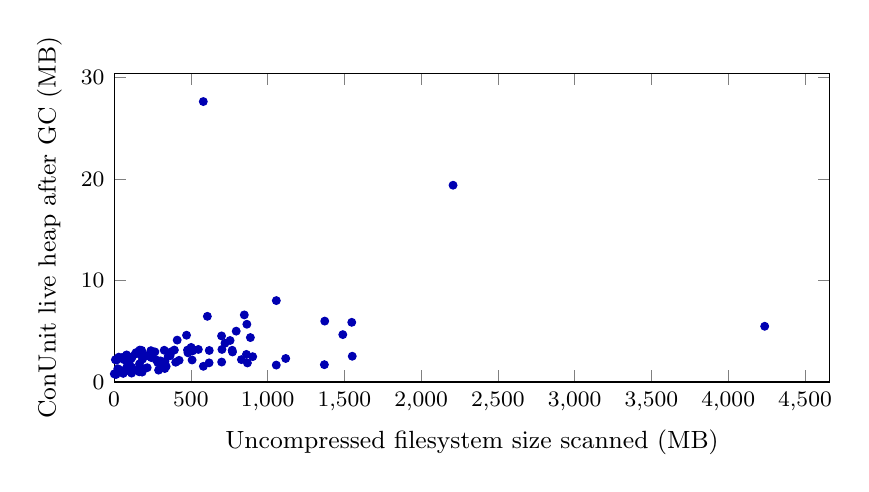
\begin{tikzpicture}
\begin{axis}[
    width=0.88\columnwidth,
    height=5.5cm,
    xlabel={Uncompressed filesystem size scanned (MB)},
    ylabel={ConUnit live heap after GC (MB)},
    xmin=0, ymin=0,
    tick label style={font=\footnotesize},
    label style={font=\small},
]
\addplot[only marks, mark=*, mark size=1.4pt, blue!70!black] coordinates {
    (1.18,0.80)
    (8.03,0.83)
    (8.28,2.20)
    (12.38,0.74)
    (14.89,2.16)
    (24.11,1.30)
    (26.76,1.28)
    (30.36,2.45)
    (41.60,1.12)
    (46.59,2.39)
    (59.44,0.85)
    (61.66,0.98)
    (62.54,2.45)
    (63.25,2.21)
    (63.85,1.15)
    (74.56,1.08)
    (81.47,2.67)
    (85.27,1.56)
    (100.17,1.74)
    (102.86,1.10)
    (105.74,2.43)
    (110.81,2.30)
    (114.07,0.88)
    (114.58,1.44)
    (116.85,1.33)
    (117.30,2.46)
    (137.07,2.75)
    (143.18,2.90)
    (163.34,1.01)
    (164.04,1.22)
    (165.30,1.79)
    (167.41,3.15)
    (168.17,2.99)
    (174.93,2.68)
    (176.90,2.95)
    (177.07,1.33)
    (179.02,3.12)
    (182.58,0.98)
    (185.25,2.26)
    (196.88,2.64)
    (214.75,2.60)
    (215.42,1.41)
    (239.79,3.09)
    (241.26,2.89)
    (242.10,2.41)
    (265.62,2.97)
    (274.17,2.18)
    (285.71,1.89)
    (289.67,1.17)
    (302.74,2.08)
    (323.64,1.55)
    (325.65,1.66)
    (326.43,3.13)
    (330.25,1.33)
    (331.14,2.02)
    (339.02,1.54)
    (352.74,2.54)
    (364.71,2.59)
    (371.61,2.98)
    (392.49,3.15)
    (401.21,1.95)
    (410.88,4.13)
    (423.42,2.14)
    (471.82,4.61)
    (477.99,3.15)
    (481.05,2.88)
    (501.75,3.41)
    (507.97,2.17)
    (511.25,3.07)
    (548.68,3.21)
    (580.92,27.62)
    (581.42,1.55)
    (607.42,6.47)
    (618.58,1.89)
    (619.81,3.11)
    (699.82,4.54)
    (700.65,1.97)
    (702.39,3.21)
    (722.21,3.82)
    (755.22,4.09)
    (768.98,3.13)
    (771.14,2.96)
    (795.28,5.01)
    (829.24,2.21)
    (847.95,6.61)
    (861.93,2.72)
    (864.72,5.69)
    (868.24,1.88)
    (887.60,4.38)
    (902.69,2.50)
    (1056.27,1.67)
    (1056.60,8.02)
    (1117.69,2.32)
    (1369.56,1.71)
    (1371.96,6.00)
    (1489.61,4.67)
    (1547.97,5.88)
    (1551.14,2.54)
    (2207.69,19.38)
    (4237.58,5.49)
};
\end{axis}
\end{tikzpicture}
